\documentclass[12pt]{article} % Document class

% Packages
\usepackage[utf8]{inputenc} % Input encoding
\usepackage[T1]{fontenc}    % Output encoding
\usepackage{booktabs}
\usepackage{enumitem}
\usepackage{amssymb}
\usepackage{xcolor}
\usepackage{listings}
\usepackage{graphicx} % insert picture
\usepackage{hyperref}
\usepackage{array} % adjust table space
\usepackage{amsmath} % use amsmath to write the formula


\definecolor{github-light-bg}{RGB}{255, 255, 255}
\definecolor{github-light-fg}{RGB}{3, 102, 214}
\definecolor{github-light-yellow}{RGB}{128, 102, 0}
\definecolor{github-light-orange}{RGB}{170, 0, 17}
\definecolor{github-light-purple}{RGB}{102, 51, 153}
\definecolor{github-light-cyan}{RGB}{0, 128, 128}
\definecolor{github-light-green}{RGB}{0, 128, 0}
\definecolor{github-light-red}{RGB}{204, 0, 0}

\lstdefinestyle{githublight}{
	backgroundcolor=\color{github-light-bg},
	basicstyle=\color{github-light-fg}\ttfamily,
	commentstyle=\color{github-light-green},
	keywordstyle=\color{github-light-purple},
	numberstyle=\tiny\color{github-light-fg},
	stringstyle=\color{github-light-cyan},
	identifierstyle=\color{github-light-orange},
	emphstyle=\color{github-light-red},
	emph={[2]TRUE,FALSE},
	emphstyle={[2]\color{github-light-yellow}},
	breaklines=true,
	breakatwhitespace=true,
	numbers=left,
	numbersep=5pt,
	stepnumber=1,
	showstringspaces=false,
	frame=single,
	rulecolor=\color{github-light-fg},
	framerule=0.5pt,
	tabsize=4,
	columns=flexible,
	extendedchars=true,
	inputencoding=utf8,
	upquote=true,
}

\lstset{style=githublight}

\title{Problem Set 4}
\date{Due: April 12, 2024}
\author{Applied Stats II}


\begin{document}
	\maketitle
	\section*{Instructions}
	\begin{itemize}
	\item Please show your work! You may lose points by simply writing in the answer. If the problem requires you to execute commands in \texttt{R}, please include the code you used to get your answers. Please also include the \texttt{.R} file that contains your code. If you are not sure if work needs to be shown for a particular problem, please ask.
	\item Your homework should be submitted electronically on GitHub in \texttt{.pdf} form.
	\item This problem set is due before 23:59 on Friday April 12, 2024. No late assignments will be accepted.

	\end{itemize}

	\vspace{.25cm}
\section*{Question 1}
\vspace{.25cm}
\noindent We're interested in modeling the historical causes of child mortality. We have data from 26855 children born in Skellefteå, Sweden from 1850 to 1884. Using the "child" dataset in the \texttt{eha} library, fit a Cox Proportional Hazard model using mother's age and infant's gender as covariates. Present and interpret the output.

\lstinputlisting[language=R, firstline=36,lastline=71]{PS04_answers_Chenxi.R} 

\newpage

\noindent Firstly we will get a Kaplan-Meier curve:
\begin{figure}[h]
	\centering
	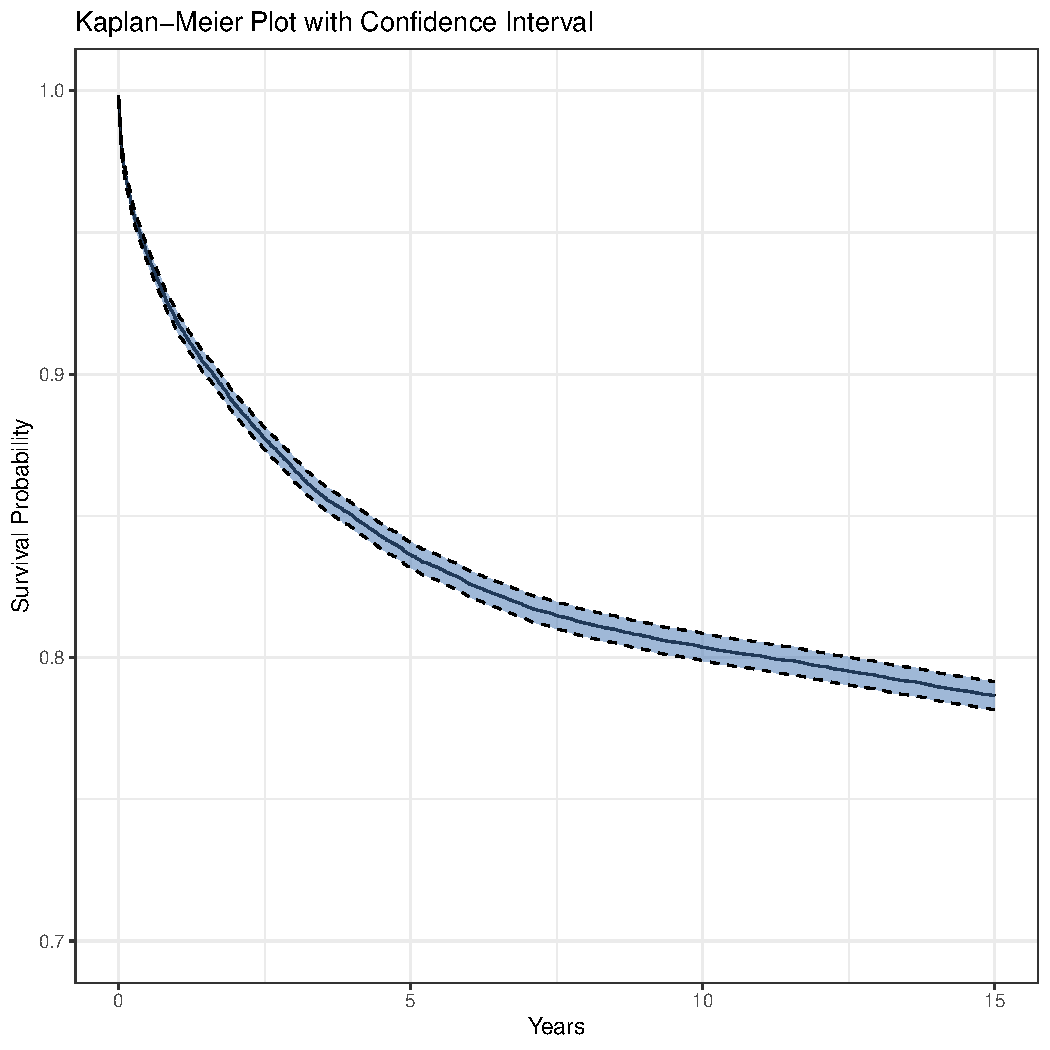
\includegraphics[scale=.5]{Kaplan-Meier.pdf} 
	\caption{Kaplan-Meier Plot}
\end{figure}

\noindent When near the 0 year, all individual haven't experience the event, so the probability of living is 1 and where the upper limit and lower limit of CI are also 1.\\
\par
\noindent With time goes by, the probability of living is decreasing and the CI is also getting wider, which means the uncertain of living probability estimation is increasing.
\newpage
\noindent And we can get our model here:
\begin{verbatim}
	Call:
coxph(formula = child_surv ~ sex + m.age, data = dat)

  n= 26574, number of events= 5616 

               coef exp(coef)  se(coef)      z Pr(>|z|)    
sexfemale -0.082215  0.921074  0.026743 -3.074 0.002110 ** 
m.age      0.007617  1.007646  0.002128  3.580 0.000344 ***
---
Signif. codes:  0 ‘***’ 0.001 ‘**’ 0.01 ‘*’ 0.05 ‘.’ 0.1 ‘ ’ 1

          exp(coef) exp(-coef) lower .95 upper .95
sexfemale    0.9211     1.0857     0.874    0.9706
m.age        1.0076     0.9924     1.003    1.0119

Concordance= 0.519  (se = 0.004 )
Likelihood ratio test= 22.52  on 2 df,   p=1e-05
Wald test            = 22.52  on 2 df,   p=1e-05
Score (logrank) test = 22.53  on 2 df,   p=1e-05
\end{verbatim}
Here are some key results:
\begin{itemize}
	\item For the exp coefficient of the sexfemale, we can interpret that compared with male, female related to a 0.92 increasing in average of the probability in risk.
	\item For the exp coefficient of the m.age, we can interpret that 1 year increase in age is associated with an increase of 1.01 on average for the probability in risk.
\end{itemize}
\end{document}
